\documentclass[a4paper, 11pt]{article}
\usepackage{fullpage} % changes the margin
\usepackage{amsmath}
\usepackage{amssymb}
\usepackage{subfig}

\usepackage{graphicx}
\graphicspath{ {../} }

\usepackage{listings}
\usepackage{color}


\definecolor{dkgreen}{rgb}{0,0.6,0}
\definecolor{gray}{rgb}{0.5,0.5,0.5}
\definecolor{mauve}{rgb}{0.58,0,0.82}

\lstset{frame=tb,
  language=Python,
  aboveskip=3mm,
  belowskip=3mm,
  showstringspaces=false,
  columns=flexible,
  basicstyle={\small\ttfamily},
  numbers=none,
  numberstyle=\tiny\color{gray},
  keywordstyle=\color{blue},
  commentstyle=\color{dkgreen},
  stringstyle=\color{mauve},
  breaklines=true,
  breakatwhitespace=true,
  tabsize=4
}

\begin{document}
	%Header-Make sure you update this information!!!!
	\noindent
	{\Huge\textbf{Graphics Assignment - 2}} \\ \\
	\Large Piyush Chauhan (1701CS33)  \hfill 28th Jan 2020\\ 

	
	\section*{Introduction}
	This task of this assignment is to draw a line with Digital Differential Analyzer(DDA) Algorithm with:
	\begin{enumerate}
		\item Symmetric DDA
		\item Simple DDA
	\end{enumerate}


	\section*{Procedure}
	
DDA is a simple algorithm. We break down the line into large number of steps. We proceed by $\Delta x$ in $x$-axis and $\Delta y$ in $y$-axis and plot the point. We do this until the end of the line is reached.

The main problem in this algorithm is choosing the step size. If we choose a small step size we repeat many pixels and waste time. If we choose a large step size we skip many pixels. The difference between the two variants of DDA is about the step size. In symmetric DDA we divide the differences by 2 until each of them is less than 1. In simple DDA we scale the differences until the largest difference is 1.

\section*{Symmetric DDA}
\subsection*{Output}
\begin{lstlisting}
	from OpenGL.GL import *
	from OpenGL.GLUT import *
	from OpenGL.GLU import *
	
	window = 0                                             # glut window number
	width, height = 500, 400                               # window size
	x1, y1, x2, y2 = list(
		map(int, input("Enter x1, y1, x2, y2 separated by spaces:").split(" ")))
	
	
	def drawLine(x1, y1, x2, y2):
		dx, dy = x2 - x1, y2 - y1
		while abs(dx) > 1 or abs(dy) > 1:
			dx /= 2
			dy /= 2
		x, y = x1, y1
		glBegin(GL_POINTS)
		glVertex2f(x, y)
		while abs(x2 - x) > 5:
			x = x + dx
			y = y + dy
			glVertex2f(x, y)
		glVertex2f(x, y)
		glEnd()
		glFlush()
	
	
	def draw():
		glClear(GL_COLOR_BUFFER_BIT | GL_DEPTH_BUFFER_BIT)  # clear the screen
		glLoadIdentity()                                   # reset position
		refresh2d(width, height)                           # set mode to 2d
		glColor3f(1.0, 1.0, 1.0)
		drawLine(x1, y1, x2, y2)
		glutSwapBuffers()
	
	
	def refresh2d(width, height):
		glViewport(0, 0, width, height)
		glMatrixMode(GL_PROJECTION)
		glLoadIdentity()
		glOrtho(0.0, width, 0.0, height, 0.0, 1.0)
		glMatrixMode(GL_MODELVIEW)
		glLoadIdentity()
	
	
	glutInit()
	glutInitDisplayMode(GLUT_RGBA | GLUT_DOUBLE | GLUT_ALPHA | GLUT_DEPTH)
	glutInitWindowSize(width, height)
	glutInitWindowPosition(250, 200)
	window = glutCreateWindow("Graphics Assignment 2")
	glutDisplayFunc(draw)
	glutIdleFunc(draw)
	glutMainLoop()
\end{lstlisting}
\subsection*{Output}
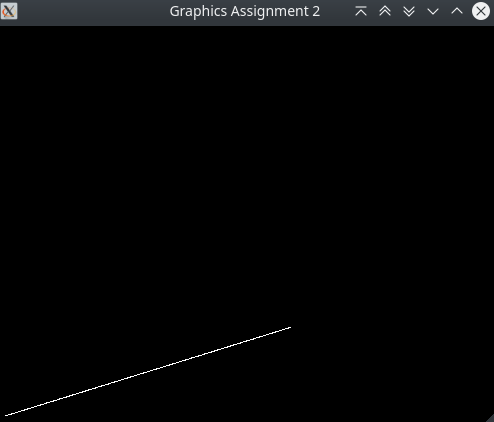
\includegraphics[width=0.48\textwidth]{symmetricDDA.png}
\captionof{figure}{Symmetric DDA}


\section*{Simple DDA}
\begin{lstlisting}
	from OpenGL.GL import *
	from OpenGL.GLUT import *
	from OpenGL.GLU import *
	
	window = 0                                             # glut window number
	width, height = 500, 400                               # window size
	x1, y1, x2, y2 = list(
		map(int, input("Enter x1, y1, x2, y2 separated by spaces:").split(" ")))
	
	
	def drawLine(x1, y1, x2, y2):
		dx, dy = x2 - x1, y2 - y1
		step = abs(dx) if abs(dx) > abs(dy) else abs(dy)
		Xin = dx/step
		Yin = dy/step
		x, y = x1, y1
		glBegin(GL_POINTS)
		glVertex2f(x, y)
	
		for i in range(int(step)):
			x = x + Xin
			y = y + Yin
			glVertex2f(x, y)
		glEnd()
		glFlush()
	
	
	# ondraw is called all the time
	def draw():
		glClear(GL_COLOR_BUFFER_BIT | GL_DEPTH_BUFFER_BIT)  # clear the screen
		glLoadIdentity()                                   # reset position
		refresh2d(width, height)                           # set mode to 2d
	
		glColor3f(0.0, 0.0, 1.0)                           # set color to blue
	
		drawLine(x1, y1, x2, y2)
	
		# important for double buffering
		glutSwapBuffers()
	
	
	def refresh2d(width, height):
		glViewport(0, 0, width, height)
		glMatrixMode(GL_PROJECTION)
		glLoadIdentity()
		glOrtho(0.0, width, 0.0, height, 0.0, 1.0)
		glMatrixMode(GL_MODELVIEW)
		glLoadIdentity()
	
	
	# initialization
	glutInit()                                             # initialize glut
	glutInitDisplayMode(GLUT_RGBA | GLUT_DOUBLE | GLUT_ALPHA | GLUT_DEPTH)
	glutInitWindowSize(width, height)                      # set window size
	# set window position
	glutInitWindowPosition(250, 200)
	# create window with title
	window = glutCreateWindow("Graphics Assignment 2")
	# set draw function callback
	glutDisplayFunc(draw)
	glutIdleFunc(draw)                                     # draw all the time
	glutMainLoop()                                         # start everything
	
\end{lstlisting}
\subsection*{Output}
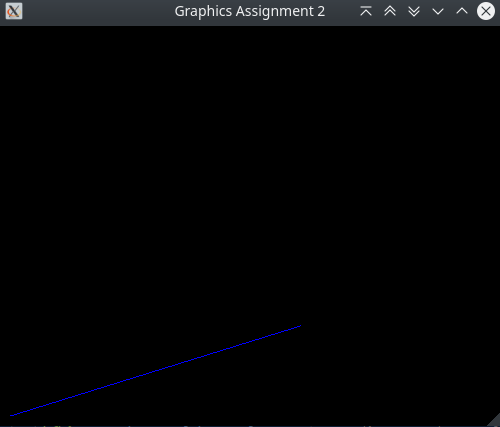
\includegraphics[width=0.48\textwidth]{simpleDDA.png}
\captionof{figure}{Simple DDA}

\end{document}